\documentclass{article}

\usepackage{fullpage}
\usepackage{amsmath}
\usepackage{amssymb}
\usepackage{graphicx} 
% \marginparwidth = 35pt
\usepackage[norsk]{babel}              % norske navn rundt omkring
\usepackage[T1]{fontenc}              % gir tilgang til alle tegn i fonten
\usepackage[utf8]{inputenc}         % utf8 rules them ALL
\usepackage{parskip}
\usepackage{multirow}
\usepackage{listings}
\usepackage[table]{xcolor}
\usepackage{fancyhdr}
\usepackage{hyperref}

% forside 
\newcommand{\PageTitle}{Detaljert Brukermanual}
\newcommand{\DateDeadline}{\today}

% SAKSMACRO
\newcommand{\sak}[2]{\section*{Sak #1: #2}}

% Bildemakro 
\def\imagetop#1{\vtop{\null\hbox{#1}}}



\begin{document}
% Importert fra fil 
\newcommand{\HRule}{\rule{\linewidth}{0.5mm}}
\begin{titlepage}
	\vspace*{3cm}
	\begin{center}
		{\Large RMI med prosjekt i distribuerte systemer TDAT3014}
		\HRule \\[0.5cm]
		{\LARGE\textsc{\textbf{\PageTitle}}}
		\HRule \\[1.0cm]
		{\large \DateDeadline} 
		\vspace{\fill}
		\begin{flushleft}
		\emph{Gruppemedlemmer}:\\
			{Andreas Mosti, \ Thomas Mowatt} 
		\end{flushleft}
	\end{center}
\end{titlepage}



\newpage
.\vfill
\begin{centering}
\LARGE


\textit{Et dokument om}  \\ 
\ \textit {Simple Network Server -} \\ 
\ \textit {Produktet}
\vspace{12cm}
\hspace{15cm}
\newpage
\end{centering} 
\fancyhead[L]{
Simple Network Server		\hfill			 Version: 1.0 \\
Kravdokument 	\hfill			Date: \today  \\}
\pagestyle{fancy}
\setlength\headsep{30pt}


\begin{table}[h] % http://en.wikibooks.org/wiki/LaTeX/Tables

\caption{Revisjonshistorikk}
	\begin{tabular}{| m{3cm} | m{1cm} | m{5cm} | m{4cm} |} 
	\hline	
	Dato & Versjon & Beskrivelse & Forfatter\\ 
	\hline
	 02/02/13> & 1.0 & Established requirements document & Andreas Mosti og Thomas Mowatt\\ 
	\hline
	<25/02/13> & 1.1 & Edited document according to the feedback & Andreas Mosti og Thomas Mowatt\\ 
	\hline
	<28/04/13> & 1.2 & Final version & Andreas Mosti og Thomas Mowatt\\ 
	\hline
	
	\end{tabular}
\end{table}

\newpage

\tableofcontents
\newpage
\section{Introduksjon}
\subsection{Mål}
Dette dokumentet er ment som brukermanual for Simple Network Server - produktet. Det vil inneholde alt som trengs for å kunne bruke løsningen fullt ut, inkludert avhengigheter og oppsett.
\subsection{Omfang}
Dette dokumentet omhandler bruk av hele systemet. \\ Beskrevet miljø er Linux (Debian - basert) og Mac OS X 10.9.
\\ MERK: Prosjektet er tilgjengelig for Windows, men dette er ikke testet. 
\subsection{Definisjoner, akronymer, forkortelser}
\begin{itemize}
\item SNS: Simple Network Server
\item SSH: Secure Shell
\item OS: Operating System
\end{itemize}
\\
\subsection{Referanser}
\begin{itemize}
\item{Mitchell Hashimoto, Vagrant: Up and Running}
\item Visjonsdokument, Kravdokument og Arkitekturdokument
\item Se fotnoter
\end{itemize}
\subsection{Innholdsoversikt}
\section{Kort om Simple Network Server}
Simple Network Server (SNS) er et ferdig, utvidbart virtuelt servermiljø basert på Ubuntu Linux som inneholder programmvare og verktøy tilpasset faget LV473D -Nettverkssikkerhet. 
\section{Testoppsett}
Denne manualen er skrevet ut ifra gjennomgang og bruk på våre testoppsett og fungerer 100\%. Disse er idag: 
\begin{itemize}
\item MacBook Pro Retina 13'', OS X  ''Maverics'' 10.9.1, 64 bit
\item Debian ''Wheezy'' 3.2.51-1, 64 bit
\item Ubuntu ''Precise Pangolin'' 12.04LTS, 32 bit
\item Ubuntu ''Precise Pangolin'' 12.04LTS, 64 bit
\item Ubuntu ''Saucy Salamander' 13.10, 64 bit
\end{itemize}
\section{Installasjon og grunnoppsett}
For å ta i bruk Simple Network Server - oppsettet for første gang må man først installere to avhengigheter samt hente ned prosjektet. Vi begynner programvare som kreves:
\subsection{Virtualbox}
Siden SNS er en virtuell løsning, må virtualiseringsløsningen virtualbox tas i bruk. Virtualbox er gratis, og kan lastes ned via \url{https://www.virtualbox.org/wiki/Download_Old_Builds} for Linux og Mac. Pakken kan også lastes rett fra pakkerepoet til Debian / Ubuntu: \\ 
\begin{lstlisting}
sudo apt-get install virtualbox
\end{lstlisting}
\\
Eller via macports\footnote{https://www.macports.org/} på OS X:
\begin{lstlisting}
sudo port install virtualbox
\end{lstlisting}
\\
Testet og anbefalt versjon er virtualbox 4.1.18. 
\subsection{Vagrant}
Den neste nødvendige programmvaren er Vagrant. Vagrant er det virtuelle miljøet SNS benytter for å kjøre, og er ment for å lage virtuelle utviklermiljøer som fokuserer på å skape like utvikleroppsett for alle som jobber på et delt prosjekt, ved bruk av vagrant vil prosjektets oppsett se likt ut for alle som tar det i bruk. Som utviklerne av Vagrant selv beskriver det: 
\begin{quote}
''Vagrant is a tool for building complete development environments. With an easy-to-use workflow and focus on automation, Vagrant lowers development environment setup time, increases development/production parity, and makes the ''works on my machine'' excuse a relic of the past.''
\end{quote}
For å installere Vagrant, last ned fra \url{http://downloads.vagrantup.com} for Linux og Mac. \\
 Pakken kan også lastes rett fra pakkerepoet til Debian / Ubuntu: \\ 
\begin{lstlisting}
sudo apt-get install vagrant
\end{lstlisting}
\\
Eller via macports på OS X:
\begin{lstlisting}
sudo port install vagrant
\end{lstlisting}
\\
Testet og anbefalt versjon av vagrant er 1.2.7. 
\footnote{Vagrant: Up and Running av vagrantskaper Mitchell Hashimoto kan eventuelt brukes som støttelitteratur. }

\subsection{Kildekode}
Selve kildekoden til SNS hentes fra github for enklest installasjon: 

\begin{lstlisting}
git clone https://github.com/andmos/SNS
\end{lstlisting}
\\
Nå kjøres prosjektet for første gang enkelt: 
\begin{lstlisting}
cd SNS/
vagrant up
\end{lstlisting}
\\ \\
Et virtuelt Ubuntu - image vil nå lastes ned (skjer kun ved første gangs kjøring) og prosjektfilene vil settes opp på dette imaget. 
Skjermbildet ved første gangs innhenting av image ser slik ut: \\ \\
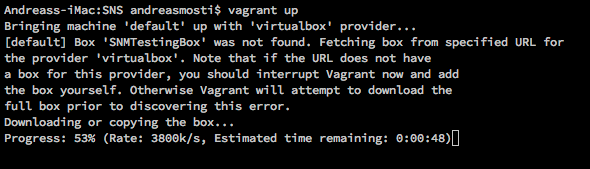
\includegraphics[scale = 0.7]{vagrantFirstTime.png}
\\ \\
Dette imaget er det vagrant kaller en ''box''. Den fungerer som grunnimage, og nedlastning skjer som sagt kun ved første gangs bygg av prosjektet. Ved alle nyoppsett av systemet vil imaget brukes som grunn-OS for prosjektfilene til SNS, eller en såkalt ''sandbox''. Boksen kan lokaliseres i den skjulte mappa ''./vagrant.d'' på hjemmekatalogen til brukeren din. \\ \\
For å sjekke at den virtuelle maskinen fungerer som den skal, gå til \url{http://localhost:8080/} fra nettleseren din. Du vil da få opp denne siden:
\\ \\
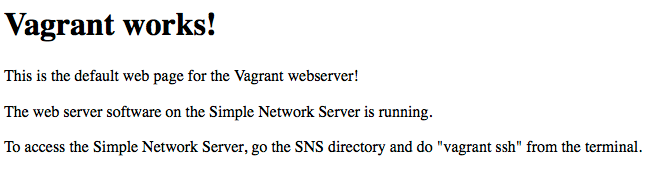
\includegraphics[scale = 0.7]{vagrantWorks.png} 
\\ \\

\subsection{Kjente oppsettsproblemer}
Den eneste feilen som har oppstått under testing er at versjonene av Virtualbox og Vagrant som ligger i repoene har vært ikke-kompatible med hverandre. Skulle dette oppstå ved oppsett, må man manuelt laste ned Virtualbox versjon 4.1.18 og legge denne inn. For 32 bit: 
\begin{lstlisting}
wget http://download.virtualbox.org/virtualbox/4.1.18/
virtualbox-4.1_4.1.18-78361~Ubuntu~precise_i386.deb
sudo dpkg -i virtualbox-4.1_4.1.18-78361~Ubuntu~precise_i386.deb
\end{lstlisting}
Og for 64 bit:
\\ 
\begin{lstlisting}
wget http://download.virtualbox.org/virtualbox/4.1.18/
virtualbox-4.1_4.1.18-78361~Ubuntu~precise_amd64.deb
sudo dpkg -i virtualbox-4.1_4.1.18-78361~Ubuntu~precise_amd64.deb
\end{lstlisting}
\\ 
Merk: Dette er pakker for Ubuntu 12.04 LTS. For andre versjoner av OS X / Linux, last ned fra \\
\url{https://www.virtualbox.org/wiki/Download_Old_Builds_4_1}
\\ \\ \\
Skulle problemer med Vagrant oppstå, kan også denne installeres utenom pakkesystemet. Da kjøres følgende (32 bit): 
\begin{lstlisting}
wget http://files.vagrantup.com/packages/7ec0ee1d00a916f80b109a298bab08e391945243/
vagrant_1.2.7_i686.deb 
sudo dpkg -i vagrant_1.2.7_i686.deb 
\end{lstlisting}
\\
Og for 64 bit - versjonen: 
\begin{lstlisting}
wget http://files.vagrantup.com/packages/7ec0ee1d00a916f80b109a298bab08e391945243/
vagrant_1.2.7_x86_64.deb
sudo dpkg -i vagrant_1.2.7_x86_64.deb
\end{lstlisting}
\\ 
Igjen, dette er pakker for Ubuntu. For andre distroer og OS X, besøk \\
\url{https://downloads.vagrantup.com/tags/v1.2.7} \\ \\
Erfaringer under testing har knyttet kjente problemer opp mot Virtualbox, så begynn med den.
\section{Arbeidsflyt}
Arbeidsflyten for produktet er veldig enkel. Når man står i prosjektets mappe, startes den virtuelle maskinen enkelt ved \\
\begin{lstlisting}
vagrant up
\end{lstlisting}
\\ 
Og maskinen aksesseres via SSH ved
\begin{lstlisting}
vagrant ssh
\end{lstlisting}
\\
Man blir da møtt av følgende skjermbilde: \\ \\
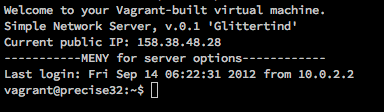
\includegraphics[scale = 0.7]{vagrantSSH.png}
\\ \\
og kan nå bruke alle verktøyene SNS tilbyr enkelt via kommandolinja, hovedsaklig via ''meny'' kommandoen for enkelhets skyld. Det er vert å merke seg at SNS - maskinen er en fullverdig virtuell Ubuntu - maskin, så all Linux - funksjonalitet utenfor prosjektets verktøy kan fritt brukes og / eller installeres. \\ 
Når man er ferdig med maskinen, avslutter man SSH - sesjonen og skriver: \\
\begin{lstlisting}
vagrant destroy
\end{lstlisting}
\\
Alle endringer og oppsett på den virtuelle maskinen blir nå slettet. Har man foreks. rotet det til med filer, angrepet serveren slik at den ikke lengre kan brukes fullstendig eller liknende, er ikke det noe problem. Nåværende system slettes. For neste gangs bruk av SNS, kjører man enkelt og greit ''vagrant up'' igjen, og prosjektet settes opp på nytt fra bunn av. 

\section{Om kildekodens oppbyggning}
<her kommer beskrivelse av mappestruktur>

\end{document}